% Created 2019-02-08 ven. 20:20
% Intended LaTeX compiler: pdflatex
\documentclass[11pt]{article}
\usepackage[utf8]{inputenc}
\usepackage[T1]{fontenc}
\usepackage{graphicx}
\usepackage{grffile}
\usepackage{longtable}
\usepackage{wrapfig}
\usepackage{rotating}
\usepackage[normalem]{ulem}
\usepackage{amsmath}
\usepackage{textcomp}
\usepackage{amssymb}
\usepackage{capt-of}
\usepackage{hyperref}
\usepackage{minted}
\usepackage[french]{babel}
\usepackage[x11names]{xcolor}
\hypersetup{linktoc = all, colorlinks = true, urlcolor = DodgerBlue4, citecolor = PaleGreen1, linkcolor = black}
\usepackage[left=1cm,right=1cm,top=2cm,bottom=2cm]{geometry}
\author{Raoul HATTERER}
\date{\today}
\title{Traitement d'image\\\medskip
\large (compléments d'informations à destination du professeur)}
\hypersetup{
 pdfauthor={Raoul HATTERER},
 pdftitle={Traitement d'image},
 pdfkeywords={},
 pdfsubject={},
 pdfcreator={Emacs 26.1 (Org mode 9.2)}, 
 pdflang={French}}
\begin{document}

\maketitle
\setcounter{tocdepth}{1}
\tableofcontents

Source : \href{http://www.ac-grenoble.fr/disciplines/informatiquelycee/n\_site/snt\_photo\_transImg.html}{Traitement d'image de l'académie de grenoble}



\section{Codage RVB et niveau de gris}
\label{sec:org945617e}

\begin{itemize}
\item Aller sur \href{https://www.w3schools.com/colors/colors\_rgb.asp}{colors RGB} et tester ce que l'on obtient si l'on remplace chacune des valeurs R, V et B d'un pixel par la moyenne des sous-pixels.
\item Essayer pour plusieurs couleurs.
\end{itemize}


\section{Images de départ}
\label{sec:orgab761a6}

Le professeur propose une ou plusieurs images couleurs de départ.

\begin{figure}[htbp]
\centering
\includegraphics[width=7cm]{pomme.jpg}
\caption{Image de départ (Pomme Linux)}
\end{figure}



\begin{figure}[htbp]
\centering
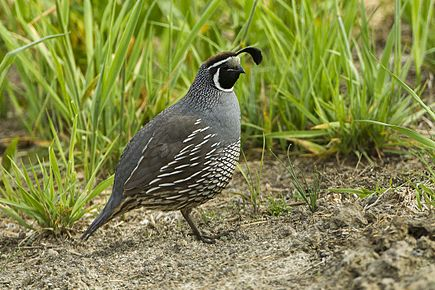
\includegraphics[width=7cm]{California_Quail.jpg}
\caption{Image de départ (Colin de Californie)}
\end{figure}


\section{Comment lire un pixel}
\label{sec:orgb51d78c}

\subsection{Installation de PIL}
\label{sec:org34983e6}

À faire au préalable par le professeur.

\begin{minted}[]{shell}
 pip3 install pillow
\end{minted}

\subsection{Activité}
\label{sec:orgd98b160}

Après avoir fait quelques recherches sur ce qu'est un "pixel", voyons comment lire le pixel de coordonnées (100,250).

\begin{minted}[]{python}
from PIL import Image
img = Image.open("pomme.jpg")
r,v,b=img.getpixel((100,250))
print("canal rouge : ",r,"canal vert : ",v,"canal bleu : ",b)
\end{minted}

\begin{verbatim}
('canal rouge : ', 19, 'canal vert : ', 88, 'canal bleu : ', 192)
\end{verbatim}


\section{Comment écrire un pixel}
\label{sec:org439882a}

\subsection{Code}
\label{sec:orga965665}

\begin{minted}[]{python}
from PIL import Image
img = Image.open("pomme.jpg")
img.putpixel((5,5),(255,0,0))
img.show()
\end{minted}

\subsection{Question}
\label{sec:org512cef8}
Identifier où se trouve l'origine de l'image.

\subsection{Réponse}
\label{sec:org719d14c}
Les élèves  écrivent un pixel de couleur spécifique à la position (0,0) ou à proximité et cherchent en examinant l'image, près de quel coin  il apparaît. On identifie ainsi que l'origine est en haut à gauche.


\section{Que fait le programme suivant ?}
\label{sec:org5e22497}

\begin{minted}[]{python}
# coding: utf-8                              # Spécifie l'encodage (ici unicode) du code source
from PIL import Image                        # Importation de la librairie PILLOW (gestion image)
img = Image.open('pomme.jpg')                # Mise en memoire dans la variable 'img' du fichier 
#                                            # pomme.jpg qui doit être dans le même répertoire que
#                                            # le programme
largeur_image,hauteur_image=img.size         # Python autorise les affectations multiples.
#                                            # img.size est un attribut (une variable intrinsèque
#                                            # à la variable img) avec les dimensions de l'image
#                                            # sous forme de tupple (= liste non modifiable). 

for y in range(hauteur_image):               # Boucle pour parcourir les toutes les lignes
    for x in range(largeur_image):           # Boucle imbriquée pour parcourir les pixels de la
        #                                    # ligne en cours
        rouge,vert,bleu=img.getpixel((x,y))  # Méthode getpixels() appliquée à la variable img qui
        #                                    # renvoie les valeurs R,V,B du pixel à la position x,y
        nouveau_rouge=vert                   # Le vert prend l'intensité du rouge
        nouveau_vert=bleu                    # Le bleu prend l'intensité du vert
        nouveau_bleu=rouge                   # Le rouge prend l'intensité du bleu
        img.putpixel((x,y),(nouveau_rouge,nouveau_vert,nouveau_bleu)) # Méthode putpixel()
#                                            # qui remplace les valeurs R, V, B du pixel en x,y 

img.show()                                   # Affichage de l'image
img.save("pommeMystere.jpg")                 # Sauvegarde de l'image obtenue
print(img.size)                              # Affichage du tupple avec la taille de l'image 
\end{minted}

\begin{verbatim}
(480, 300)
\end{verbatim}


On analyse le code ci-dessus (sans forcément rentrer dans les détails) qui servira de base pour le défi suivant.

\begin{figure}[htbp]
\centering
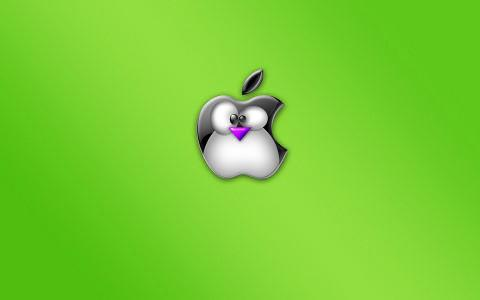
\includegraphics[width=7cm]{pommeMystere.jpg}
\caption{Résultat du programme mystère}
\end{figure}

Les couleurs ont été permutées.


\section{Passage d'une image en niveaux de gris (codé RVB sur 3 octets)}
\label{sec:org8fb882e}

Après avoir fait quelques recherches sur les "images en niveaux de gris", écrivez un programme qui transforme une "image couleur" en une "image en niveaux de gris".

Petite astuce qui pourrait vous aider : en Python pour avoir une division entière (le résultat est un entier), il faut utiliser l'opérateur // à la place de l'opérateur / 

Remarque: On donne l'algorithme aux élèves (ou on le construit avec eux) ; ils doivent alors programmer le passage d'une image couleur à une image en niveaux de gris.


\begin{minted}[linenos,firstnumber=1]{python}
from PIL import Image
img = Image.open("pomme.jpg")
largeur_image,hauteur_image=img.size

for y in range(hauteur_image):
    for x in range(largeur_image):
       rouge,vert,bleu=img.getpixel((x,y))
       nouveau_rouge=(vert+bleu+rouge)//3
       nouveau_vert=(vert+bleu+rouge)//3
       nouveau_bleu=(vert+bleu+rouge)//3
       img.putpixel((x,y),(nouveau_rouge,nouveau_vert,nouveau_bleu))

img.show()
img.save("pommegrise.jpg")
\end{minted}

\begin{figure}[htbp]
\centering
\includegraphics[width=7cm]{pommegrise.jpg}
\caption{Pomme Linux en niveaux de gris (codé RVB)}
\end{figure}



\begin{minted}[linenos,firstnumber=1]{python}
from PIL import Image
img = Image.open("California_Quail.jpg")
largeur_image,hauteur_image=img.size

for y in range(hauteur_image):
    for x in range(largeur_image):
       rouge,vert,bleu=img.getpixel((x,y))
       nouveau_rouge=(vert+bleu+rouge)//3
       nouveau_vert=(vert+bleu+rouge)//3
       nouveau_bleu=(vert+bleu+rouge)//3
       img.putpixel((x,y),(nouveau_rouge,nouveau_vert,nouveau_bleu))

img.show()
img.save("colingris.jpg")
\end{minted}

\begin{figure}[htbp]
\centering
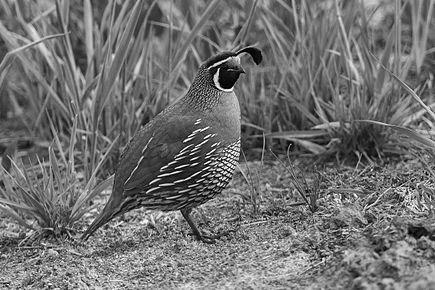
\includegraphics[width=7cm]{colingris.jpg}
\caption{Colin de Californie en niveaux de gris RVB}
\end{figure}

\section{Passage d'une image en niveau de gris (codé L sur 1 seul octet)}
\label{sec:org8e1858b}


\subsection{Utilisation du mode \texttt{L} (luminance) pour les images en nuances de gris}
\label{sec:orgb1a962a}
\subsubsection{Pomme Linux}
\label{sec:org13004af}

\begin{minted}[linenos,firstnumber=1]{python}
from PIL import Image
img = Image.open("pomme.jpg").convert("L")
img.show()
img.save("pommegriseL.jpg")
\end{minted}


\begin{figure}[htbp]
\centering

\includegraphics[width=7cm]{pommegriseL.jpg}
\caption{Image en niveaux de gris (codé L)}
\end{figure}


\subsubsection{Colin de Californie}
\label{sec:orge8ead10}

\begin{minted}[linenos,firstnumber=1]{python}
from PIL import Image
img = Image.open("California_Quail.jpg").convert("L")
img.show()
img.save("colingrisL.jpg")
\end{minted}


\begin{figure}[htbp]
\centering
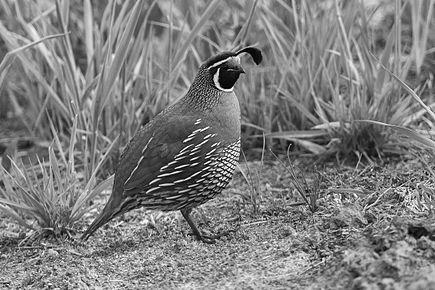
\includegraphics[width=7cm]{colingrisL.jpg}
\caption{Colin de Californie en niveaux de gris (luminance L)}
\end{figure}

Comparer la taille des différents fichiers. Conclure.



\emph{Réponse : codée avec un octet par pixel, l'image (les datas) prend moins de place donc le fichier est moins lourd (la compression jpeg atténue le phénomène).}

\subsection{Existe-t-il d'autres modes ?}
\label{sec:org35bd427}

Les \href{https://pillow.readthedocs.io/en/latest/handbook/concepts.html\#modes}{modes} supportés par \texttt{Pillow} sont : 

\begin{itemize}
\item \texttt{1} (1-bit pixels, black and white, stored with one pixel per byte)
\item \texttt{L} (8-bit pixels, black and white)
\item \texttt{P} (8-bit pixels, mapped to any other mode using a color palette)
\item \texttt{RGB} (3x8-bit pixels, true color)
\item \texttt{RGBA} (4x8-bit pixels, true color with transparency mask)
\item \texttt{CMYK} (4x8-bit pixels, color separation)
\item \texttt{YCbCr} (3x8-bit pixels, color video format)
\item \texttt{LAB} (3x8-bit pixels, the L*a*b color space)
\item \texttt{HSV} (3x8-bit pixels, Hue, Saturation, Value color space)
\item \texttt{I} (32-bit signed integer pixels)
\item \texttt{F} (32-bit floating point pixels)
\end{itemize}



\section{Récréation ou challenge ?}
\label{sec:orgc6275f8}

\subsection{Créer une image en négatif}
\label{sec:orgc024222}

\begin{minted}[linenos,firstnumber=1]{python}
from PIL import Image
img = Image.open("pomme.jpg")
largeur_image,hauteur_image=img.size

for y in range(hauteur_image):
    for x in range(largeur_image):
        rouge,vert,bleu=img.getpixel((x,y))
        nouveau_rouge=255-rouge
        nouveau_vert=255-vert
        nouveau_bleu=255-bleu
        img.putpixel((x,y),(nouveau_rouge,nouveau_vert,nouveau_bleu))

img.show()
img.save("pommeNegatif.jpg")
\end{minted}

\begin{figure}[htbp]
\centering
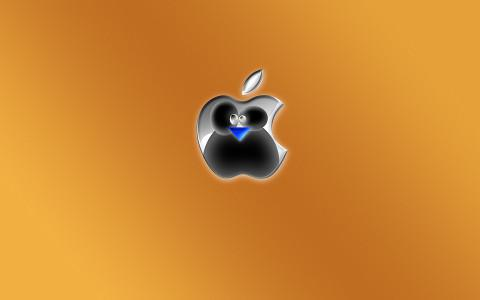
\includegraphics[width=7cm]{pommeNegatif.jpg}
\caption{Négatif}
\end{figure}

\subsection{Diagonale}
\label{sec:orgbf3e690}

Créer le programme qui garde l'image d'origine au-dessus d'une diagonale et qui transforme en niveaux de gris en-dessous de celle-ci.

\begin{minted}[linenos,firstnumber=1]{python}
from PIL import Image
img = Image.open("pomme.jpg")
largeur_image,hauteur_image=img.size

for y in range(hauteur_image):
    tailleDiag=y*largeur_image//hauteur_image
    for x in range(tailleDiag):
       rouge,vert,bleu=img.getpixel((x,y))
       nouveau_rouge=(vert+bleu+rouge)//3
       nouveau_vert=(vert+bleu+rouge)//3
       nouveau_bleu=(vert+bleu+rouge)//3
       img.putpixel((x,y),(nouveau_rouge,nouveau_vert,nouveau_bleu))

img.show()
img.save("pommemisgrise.jpg")
\end{minted}

\begin{figure}[htbp]
\centering

\includegraphics[width=7cm]{pommemisgrise.jpg}
\caption{Pomme coupée}
\end{figure}
\end{document}